% !Mode:: "TeX:UTF-8" (encoding info for WinEdt)
\section{Elexis et les Tarifs pour les médecins en Suisse }
\label{arzttarife}
Puisque Elexis est un logiciel du cabinet universelle, le Tarmed n'est qu'une des possibilités d'un système de facturation. Par conséquent ni la saisie des prestations ni la facturation elle-même fait partie du noyau du système mais se trouve dans des Plugins. Puisque Elexis est un logiciel Suisse il va de soi que ce Plugin fait partie de la distribution standard.
\subsection{Réglages}
\begin{figure}
  % Requires \usepackage{graphicx}
  \center
  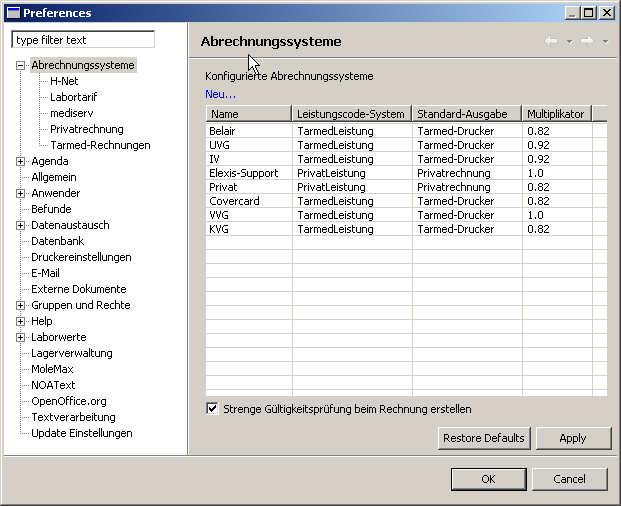
\includegraphics[width=0.9\textwidth]{images/arztrechnung1}\\
  \caption{Abrechnungssysteme}\label{fig:tarmed1}
\end{figure}

Dès que le Plugin Tarmed est installé (ce qui est selon de standard toujours le cas) vous pouvez choisir sous les systèmes de facturation  (cf. fig. \ref{fig:tarmed1}) des prestations et imprimantes Tarmed. Lors de l'établissement d'un nouveau cas les systèmes de facturation LAMAL, LAA, LAI, LCA et LAM sont installés de façon standardisée. D'autres systèmes (par ex. Covercard) peuvent être ajoutés manuellement respectivement sont ajoutés par des plugins. Des plus amples informations concernant les systèmes de facturation vous trouvez dans l'annexe sous \ref{settings:abrechnungssystem} à la page \pageref{settings:abrechnungssystem}. \textbf{Important:} N'oubliez pas d'introduire la valeur du point de taxe spécifique pour votre canton avant d'introduire les premières prestations.  Lors d'un changement de la valeur du point cantonal il ne faut pas oublier de l'adapter dans Elexis avant d'introduire des prestations qui sont concernées par le nouveau point cantonal. Des changements ultérieurs après avoir imprimé les factures sont très fastidieux. Il ne faut pas non plus oublier d'introduire sous 'Tarif du laboratoire' le point de taxe actuel.

Un point de taxe est toujours valable à partir d'une date spécifique. Il est toujours valable jusqu'à ce qu'un nouveau point de taxe est introduit. Une valeur une fois introduite ne peut plus être modifiée ou effacée (car sinon des prestations qui ont été comptabilisées avec ce point de taxe seront nulles). Par contre ont peut à tout moment introduire un nouveau point de taxe, valable à partir d'une date spécifique, en cliquant sur le bouton prévu à cette fin.
Si vous ouvrez la section Tarmed (sous 'fichiers - options') apparaît la page du réglage des factures  (Fig. \ref{fig:tarmed2}). Il y faudra régler individuellement pour chaque mandant tout les détails concernant les factures.

\begin{figure}
  % Requires \usepackage{graphicx}
  \center
  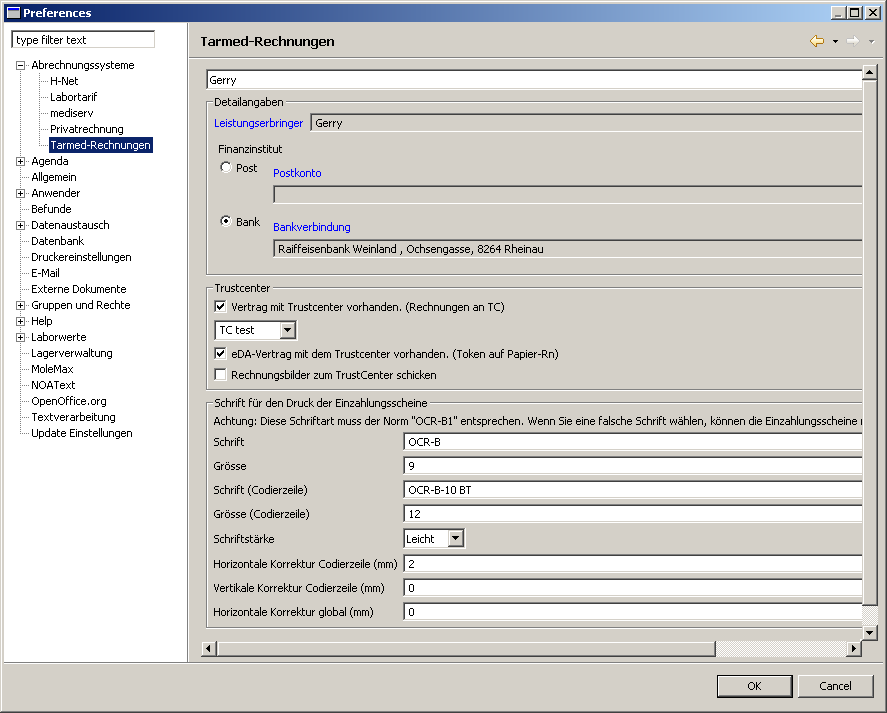
\includegraphics[width=0.9\textwidth]{images/arztrechnung2}\\
  \caption{Tarmed-Einstellungen}\label{fig:tarmed2}
\end{figure}


Choisissez dans le 'Combobox' en haut un mandant. Cliquez ensuite sur le mot prestataire. Il apparaît une liste avec tout ce que Tarmed veut savoir de vous :

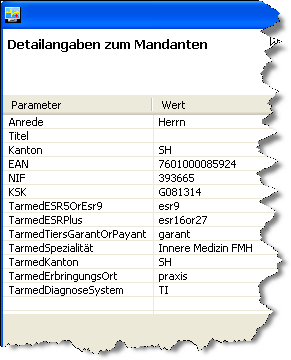
\includegraphics[width=3in]{images/tarmed3}
% tarmed3.png: 291x360 pixel, 96dpi, 7.70x9.52 cm, bb=0 0 218 270

\begin{itemize}



\item Titre - eh bien , ceci est encore facile
\item Titre professionnel - idem
\item Canton : Le canton dans lequel vous effectuez des prestations sous le nom du mandant. Si vous exercez dans plusieurs cantons vous devez créer pour chaque canton un mandant spécifique.
\item Code EAN : Tarmed dit que vous n'êtes qu'un article. Il faut introduire ici votre numéro d'article européen. Ceci doit impérativement être un numéro à 13 chiffres. .
\item NIF : L'AI dit que vous êtes un porteur de NIF (quoi que ce soit). Il faut introduire ici votre numéro NIF.
\item Numéro du concordat : SantéSuisse dit : Vous êtes porteur d'un numéro du concordat. Vous devez introduire ici votre numéro du concordat respectivement votre numéro RCC et ceci sans trait d'union. Ceci doit être toujours une lettre suivi de 6 chiffres.
\item Commentaire : Elexis a choisi dans ce contexte consciemment un design qui est aménageable. Si quelques bureaucrates devaient inventer encore un autre système de numérotation avec lequel nous devrions nous classifier une fois de plus - pas de problème. Elexis peut vous introduire dans n'importe quel nouveau système de codification. Mais continuons :
\item TarmedESR5OrEsr9- Le système ESR (un numéro de participant de 5 ou 9 chiffres).
Elle se trouve dans votre convention ESR. Normalement c'est esr9.

\item TarmedESRPlus-esr16or27 est juste lorsque vous voulez/pouvez introduire le montant dans la ligne ESR (ceci est normalement le cas), esr16or27plus vous devez déclarer, lorsque vous voulez que le client doit introduire le montant manuellement.
\item Tarmed-Spécialité : Votre titre de spécialiste avec lequel vous facturez sous ce mandant.
\end{itemize}
Cliquez ensuite selon vos préférences sur   \textit{référence bancaire} ou  \textit{compte postal}

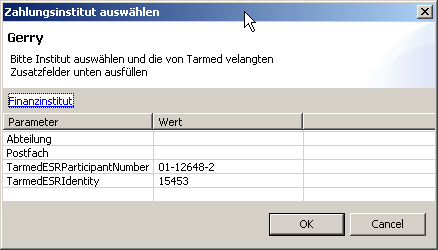
\includegraphics[width=4in]{images/tarmed4.png}
% tarmed4.png: 438x250 pixel, 96dpi, 11.59x6.61 cm, bb=0 0 328 187


Sous 'référence bancaire' vous choisissez votre banque (dont les coordonnés ont déjà été saisi sous 'contacts') par un clic sur  \glqq
établissement bancaire\grqq{}   Ensuite il faut ajouter encore deux détails au contrat-ESR : TarmedESRParticipantNumber - le numéro de participant ESR de otre Banque (renseignez-vous chez votre banque ) et TarmedESRIdentity- votre numéro de client-BESR qui doit vous être donné aussi par votre banque.

\textbf{Attention:} Vous ne pouvez pas imprimer des factures Tarmed ou envoyer des factures au Centre de confiance sans avoir introduit d'abord toutes ces données correctement. Ce n'est pas une chicane de Elexis mais les conditions de Tarmed.

\subsubsection{Réglages de l'imprimante}

Elexis utilise l'imprimante par défaut pour l'impression des factures. Pour la changer il faut choisir sous  \textit{imprimantes et télécopieurs } l'imprimante qui doit être définie (par la touche droite de la souris) comme imprimante par défaut.
Par la suite l'impression devrait se faire sur la nouvelle imprimante. On peut aussi configurer quel bac de l'imprimante doit être utilisé.

\subsection{Les Factures}

Comme déjà mentionné une facture Tarmed peut avoir des formes différentes :

\begin{itemize}
 \item une forme de fichier XML, utile pour la transmission au Centre de confiance
\item un fichier utile pour la transmission à la caisse des médecins
\item un formulaire de facturation Tarmed sur papier idéal pour les systèmes tiers payant.
\item  une page avec BVR et justificatif de remboursement pour les systèmes tiers garant.
\end{itemize}

Laquelle de toutes ces méthodes est celle qui convient dépend de votre canton, des réglages contractuelles et du cas spécifique pour lequel la facture est établi. Des cas LAA sont normalement traités en forme tiers payant tandis que des cas LAMAL sont traités dans la majorité des cantons (mais pas dans tous) en tiers garant ce qui est compliqué par le fait que certaines caisses ont crée des contrats tiers payant avec certains médecins. La conclusion est : Elexis ne peut pas vous aider dans ça mais vous fournit la forme de facture correcte si vous avez introduit les donnés correctes sous \textsc{Cas - Détail}.

\subsection{'Views' de ce Plugin}
Ce Plugin collabore avec la 'View des factures' existante dans le noyau du système. Il apporte qu'une propre View pour l'enregistrement des payements :

\subsubsection{ESR}
\begin{figure}[hb]
  % Requires \usepackage{graphicx}
  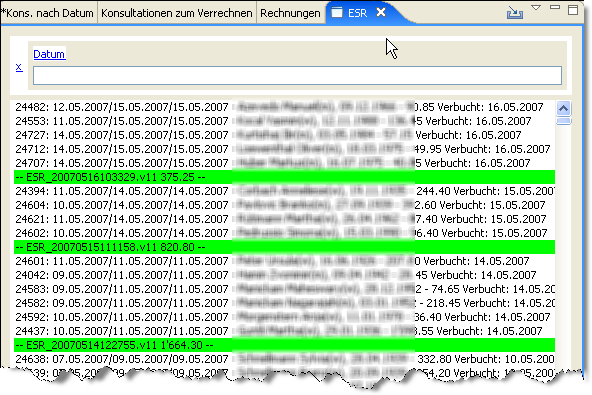
\includegraphics{images/esr1}\\
  \caption{View zum einlesen von ESR Dateien}\label{fig:esr}
\end{figure}

 Sous Fig.\ref{fig:esr} vous voyez la 'View' pour la lecture des fichiers ESR. Si vous avez signé un contrat spécifique avec votre banque, elle va vous mettre à disposition les fichiers ESR soit par une disquette soit pour le téléchargement directe 'online'. Les fichiers ESR contiennent les payements de vos factures. Elexis est capable d'introduire les fichiers ESR directement pour acquitter automatiquement les montants des factures en question.

